\mytitlepage{Прикладной математики}{2}{Комьютерная графика}{Трехмерная визуализация в режиме реального времени}{ПМ-63}{Шепрут И.И.}{-}{Задорожный А.Г.}{2019}

\section{Цель работы}

Ознакомиться с методом тиражирования сечений (основным способом задания полигональных моделей) и средствами трехмерной визуализации (системы координат, источники света, свойства материалов).

\section{Постановка задачи}

\noindent\normalsize{\begin{easylist}
\ListProperties(Hang1=true)
& Считывать из файла (в зависимости от варианта):
&& 2D-координаты вершин сечения (считающегося выпуклым);
&& 3D-координаты траектории тиражирования;
&& параметры изменения сечения.
& Построить фигуру в 3D по прочитанным данным.
& Включить режимы:
&& буфера глубины;
&& двойной буферизации;
&& освещения и материалов.
& Предоставить возможность показа:
&& каркаса объекта;
&& нормалей (например, отрезками);
&& текстур, <<обернутых>> вокруг фигуры.
& Предоставить возможность переключения между режимами ортографической и перспективной проекции.
& Обеспечить навигацию по сцене с помощью модельно-видовых преобразований, сохраняя положение источника света.
& Предоставить возможность включения/выключения режима сглаживания нормалей.
\end{easylist}}

Вариант: \textbf{\texttt{Рендеринг порталов.}}

\section{Реализованные функции}

\noindent\normalsize{\begin{easylist}
\ListProperties(Hide=100, Hang1=true, 
	Progressive*=.5cm,%	
	Style1*=\textbullet ,%
	Style2*=\textopenbullet )
& \textbf{Рендеринг порталов.} 
&& Порталы рисуются во всех возможных граничных случаях. Никаких перекрытий или артефактов во время рендеринга не появится.
& \textbf{Считывание произвольной сцены из многоугольников, с анимаций, из \texttt{json} файла.}
&& Поддержка задания анимаций в сцене.
& \textbf{Поддержка текстур.}
& \textbf{Рисование невыпуклых многоугольников.}
& Вращение камеры вокруг сцены при помощи мыши.
&& Так же имеется приближение/отдаление с помощью колесика мыши.
& Имеется меню на все основные функции.
& Рендеринг с учетом точечных источников света.
\end{easylist}}

\subsection{Для достижения всего этого, были использованы:}

\noindent\normalsize{\begin{easylist}
\ListProperties(Hide=100, Hang1=true, 
	Progressive*=.5cm,%	
	Style1*=\textbullet ,%
	Style2*=\textopenbullet )
	Библиотека \texttt{glm} для работы с матрицами и векторами.
& \texttt{ClipPlane} для удаления невидимых частей при рендеринге сцены <<внутри>> портала.
& Собственный расчет \texttt{ClipPlane} для определения того, необходимо рисовать портал или нет, так как рендеринг портала - самая дорогая по времени операция.
& Собственный расчет определения лицевых граней для рендеринга фронтальной и задней стороны портала. Опять же в целях оптимизации.
& Расчет пересечений спроецированных порталов с помощью библиотеки \texttt{clipper} при рендеринге порталов более глубокого уровня, для того чтобы определить порталы, которые точно не будут видны на экране.
& \texttt{Framebuffer}'ы с цветом и глубиной, для того, чтобы рисовать сцену каждого портала в отдельном буфере.
& Шейдеры, для того, чтобы при помощи них объединять \texttt{Framebuffer}'ы, или рисовать их на экране.
& Библиотека \texttt{stb\_image.h} для считывания изображений для текстур.
& Библиотека \texttt{nlohmann/json} для считывания и записи сцен в \texttt{json}. 
& Методы \texttt{gluTess}, для получения множества выпуклых примитивов из невыпуклого многоугольника.
\end{easylist}}

\section{Пример реализованных функций}

\subsection{Меню}

В меню так же с отступом написано как воспользоваться данной возможностью при помощи клавиатуры, а конкретно, там сказана клавиша, реализующая это действие. 

\begin{center}
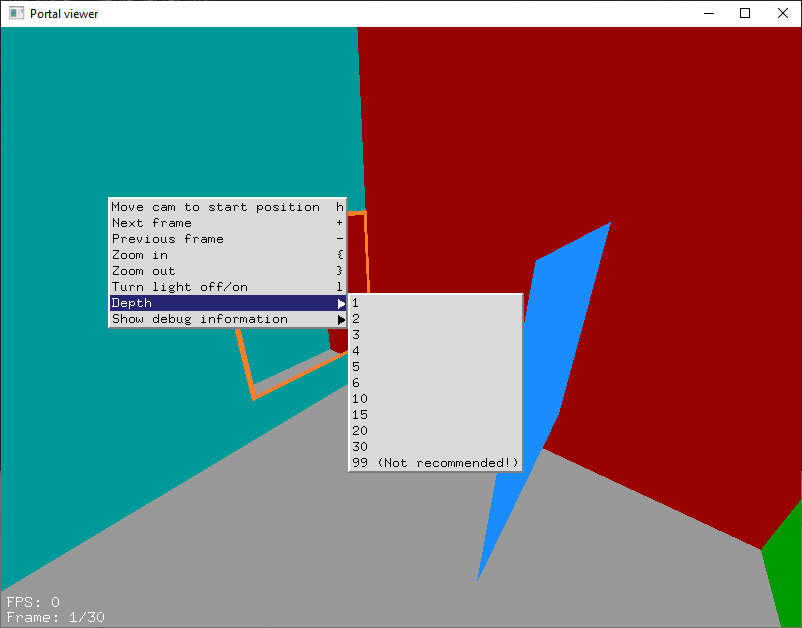
\includegraphics[width=0.75\textwidth]{img/1.png}
\end{center}

\subsection{Анимация}

Внизу можно увидеть номер текущего кадра во всей анимации.

\begin{center}
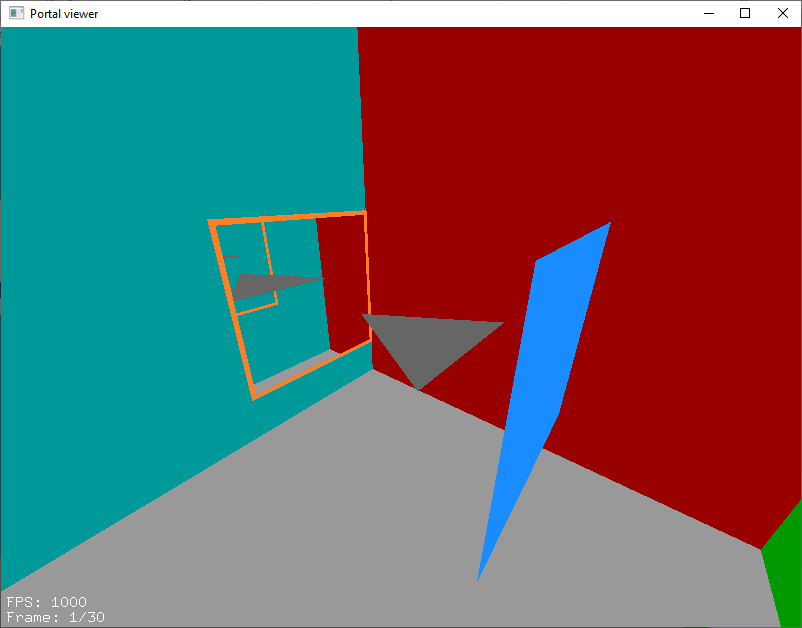
\includegraphics[width=.48\textwidth]{img/2.png}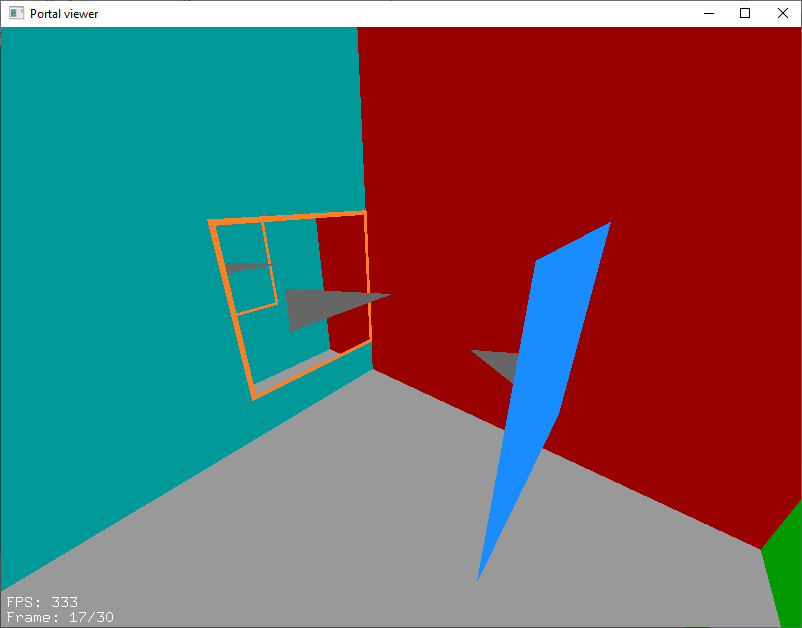
\includegraphics[width=.48\textwidth]{img/3.png}
\end{center}

\subsection{Простая сцена с порталами}

\begin{center}
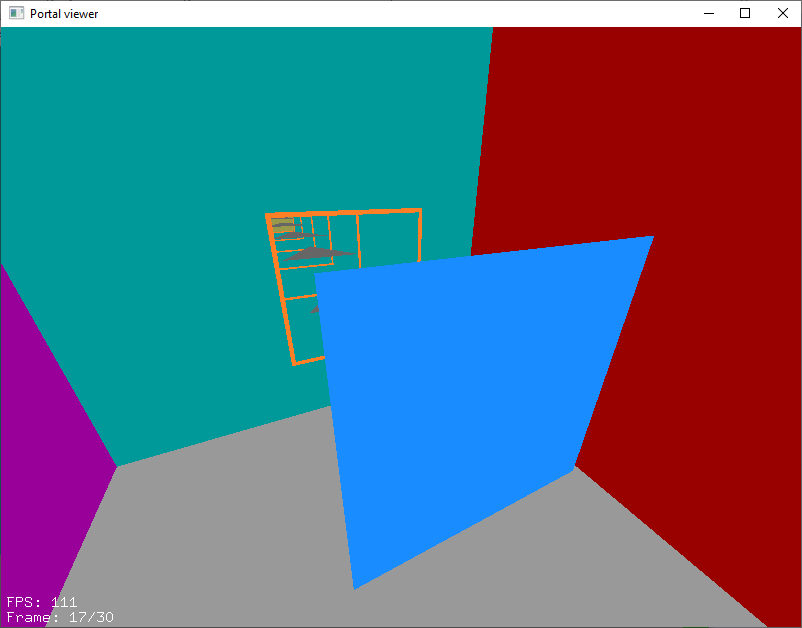
\includegraphics[width=.48\textwidth]{img/4.png}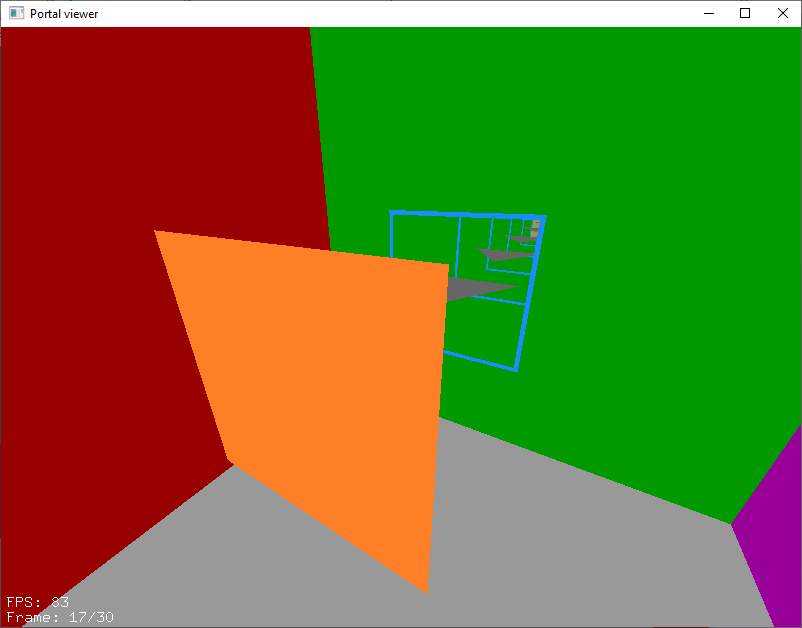
\includegraphics[width=.48\textwidth]{img/5.png}
\end{center}

\subsection{Задание большой глубины}

\begin{center}
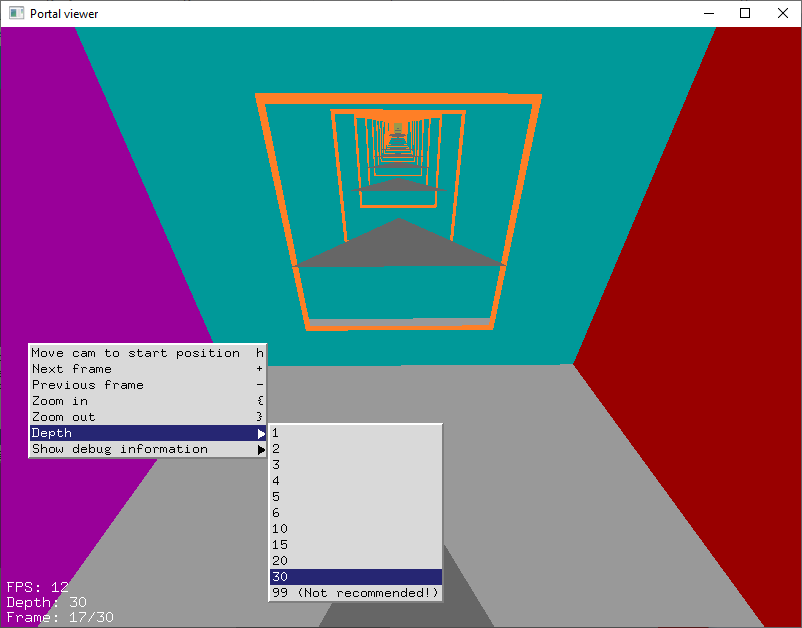
\includegraphics[width=0.75\textwidth]{img/6.png}
\end{center}

\subsection{Объёмный портал}

\textit{Примечание:} объёмный портал --- это портал, полученный соединением нескольких обычных порталов таким образом, что сохраняется непрерывность и целостность пространства. Самое главное в этом тесте, что через портал видно другую часть портала, а через неё исходную сцену.

\begin{center}
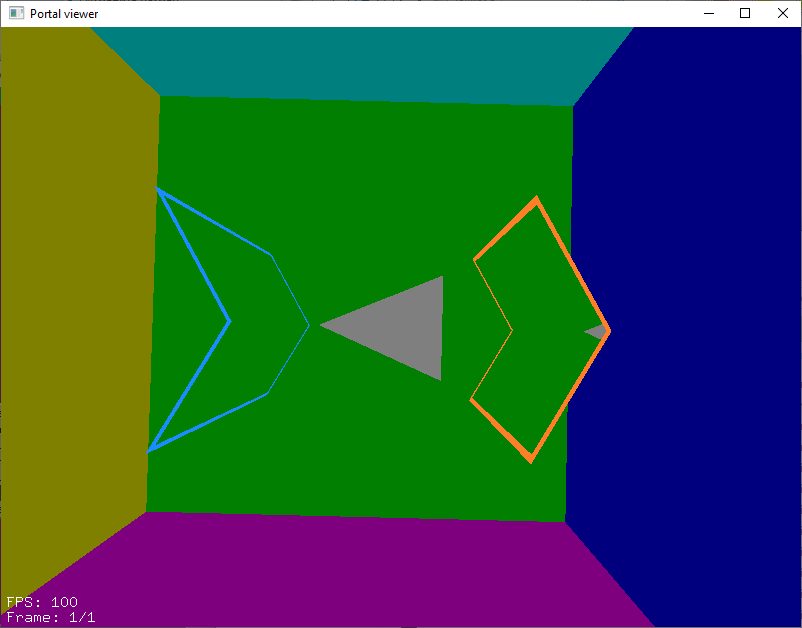
\includegraphics[width=.48\textwidth]{img/7.png}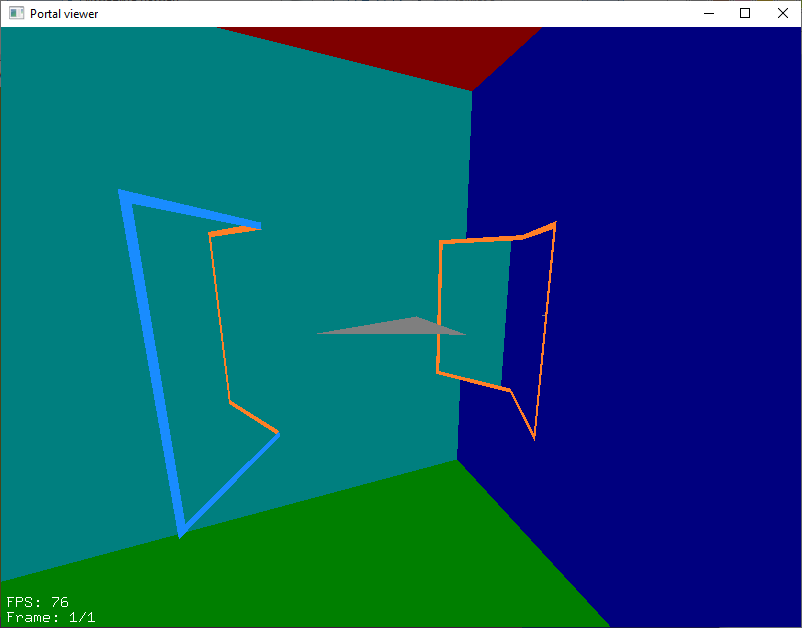
\includegraphics[width=.48\textwidth]{img/8.png}
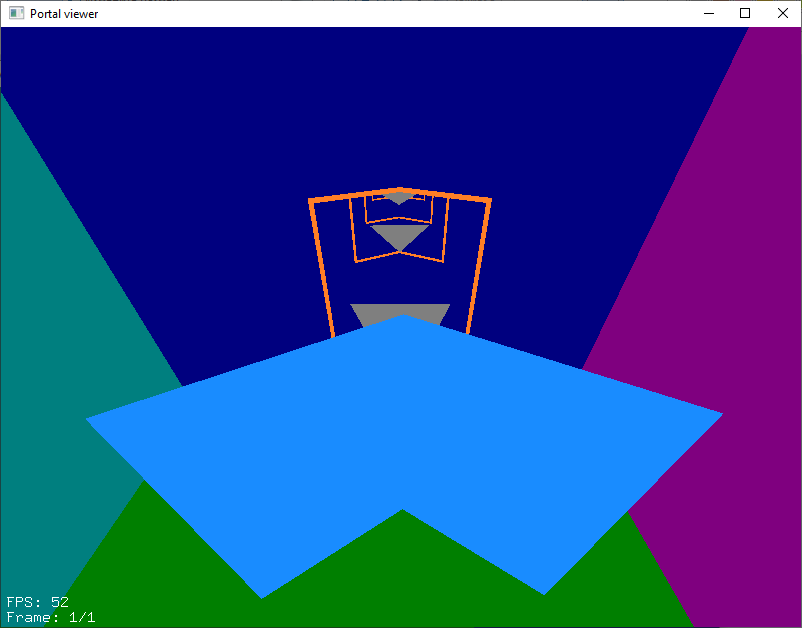
\includegraphics[width=.48\textwidth]{img/9.png}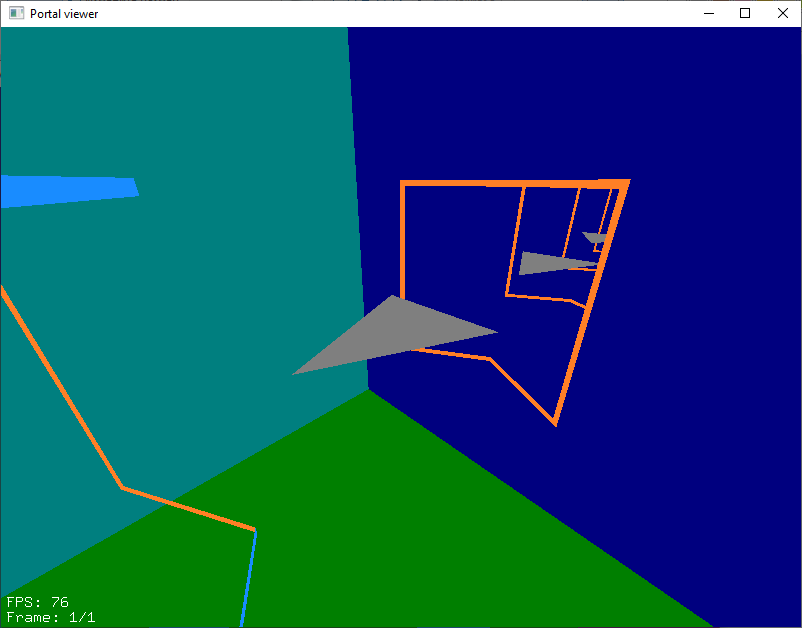
\includegraphics[width=.48\textwidth]{img/10.png}
\end{center}

\subsection{Использование текстур}

\begin{center}
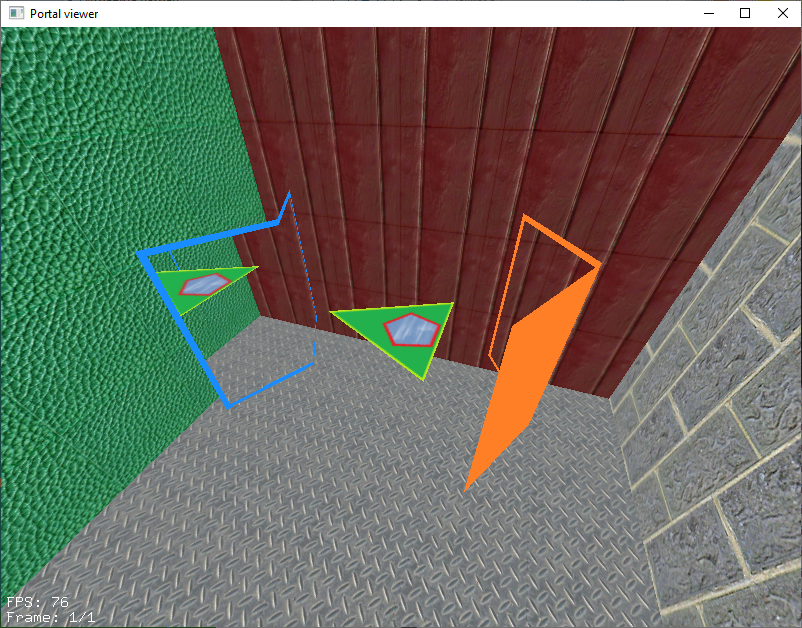
\includegraphics[width=.48\textwidth]{img/11.png}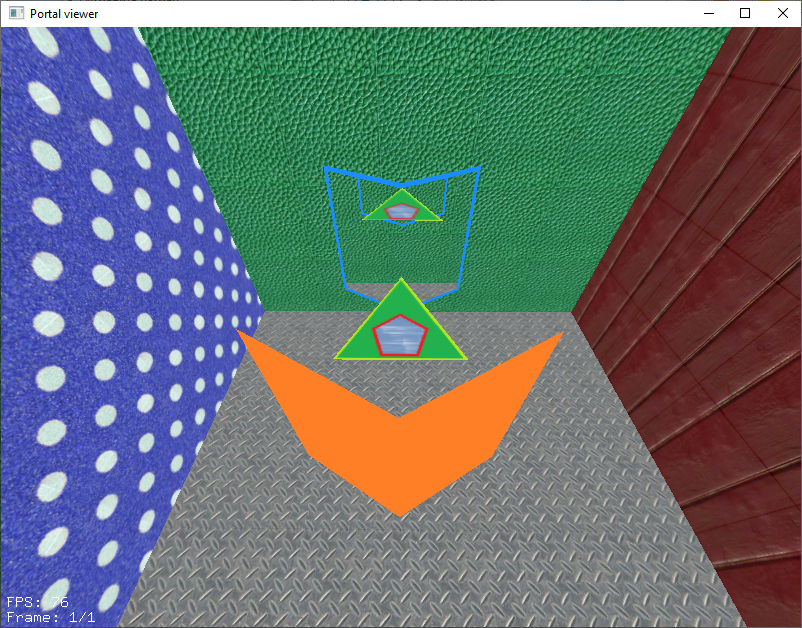
\includegraphics[width=.48\textwidth]{img/12.png}
\end{center}


\subsection{Наклоненный портал}

\begin{center}
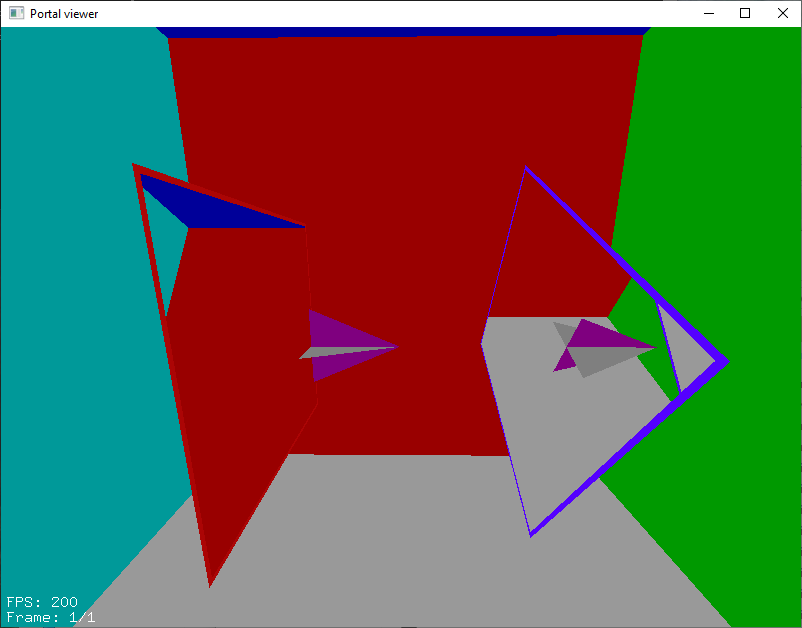
\includegraphics[width=.48\textwidth]{img/13.png}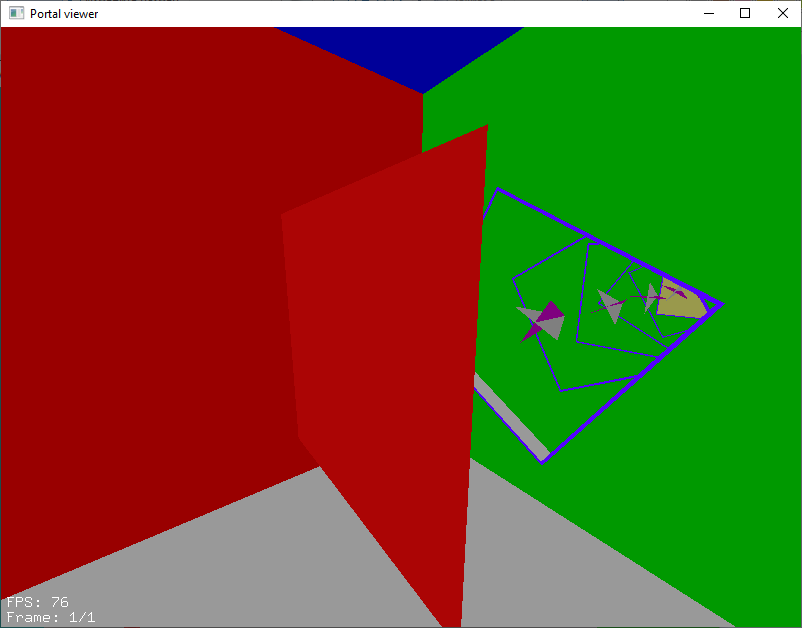
\includegraphics[width=.48\textwidth]{img/14.png}
\end{center}


\subsection{Портал, изменяющий масштаб мира}

Одна часть данного портала уменьшена по сравнению с другой, получается, всё, что войдет в этот портал, будет уменьшено, а что войдет в другой, увеличено. На данной сцене можно видеть, что в одном портале полигон уменьшается, а на другом увеличивается.

\begin{center}
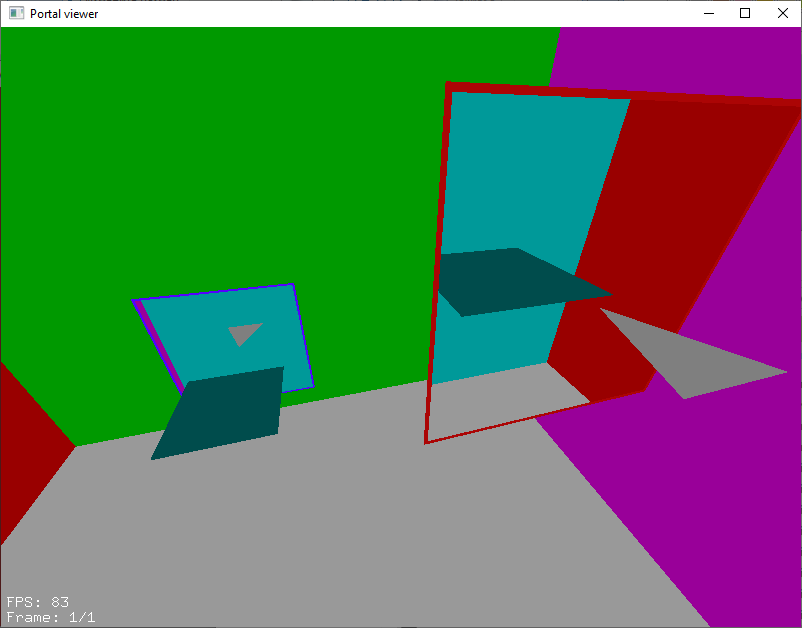
\includegraphics[width=.48\textwidth]{img/15.png}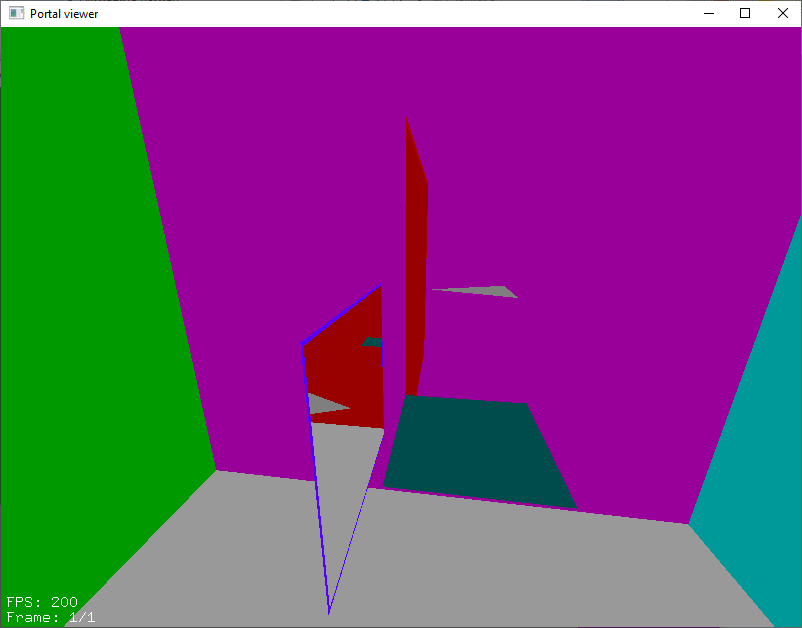
\includegraphics[width=.48\textwidth]{img/16.png}
\end{center}


\subsection{Портал, изменяющий наклон мира}

Аналогично предыдущему, только здесь одна часть наклонена относительно другой, и получается, что при просмотре из одного портала в другой, наклоняется весь мир.

\begin{center}
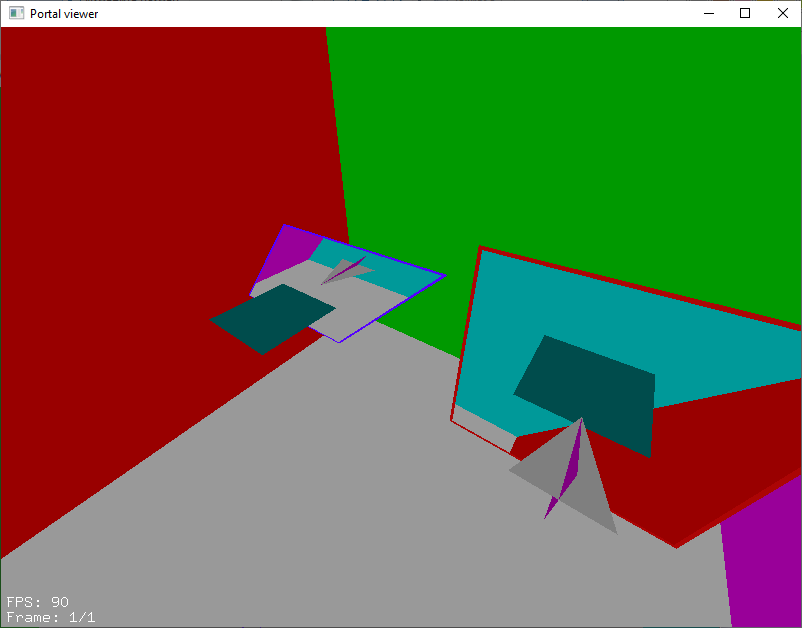
\includegraphics[width=.48\textwidth]{img/17.png}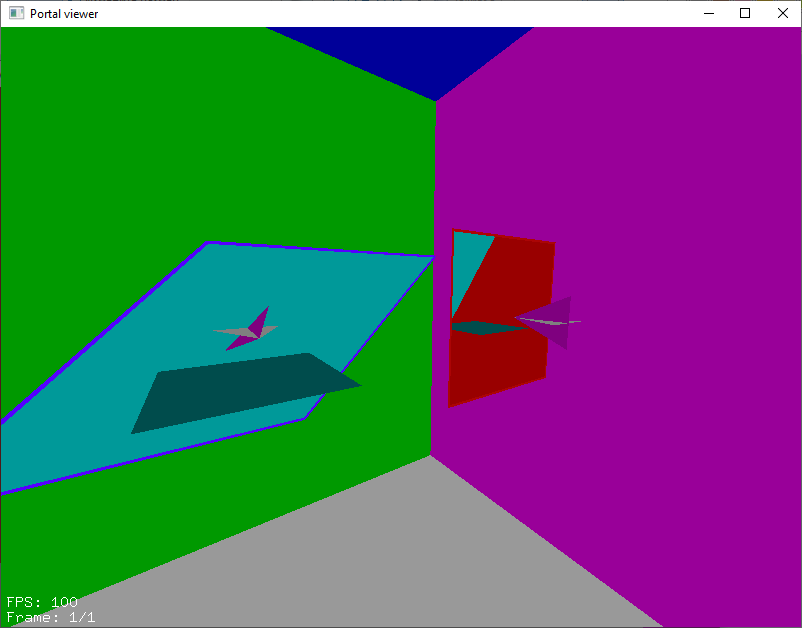
\includegraphics[width=.48\textwidth]{img/18.png}
\end{center}


\subsection{Пропеллер из порталов}

Этот тест призван показать, что никаких пересечений сцены или рендеринга между порталами нет, и они корректно работают с буфером глубины. При рендеринге порталов, считается, что вся сцена, находящаяся внутри него, рисуется как текстура.

\begin{center}
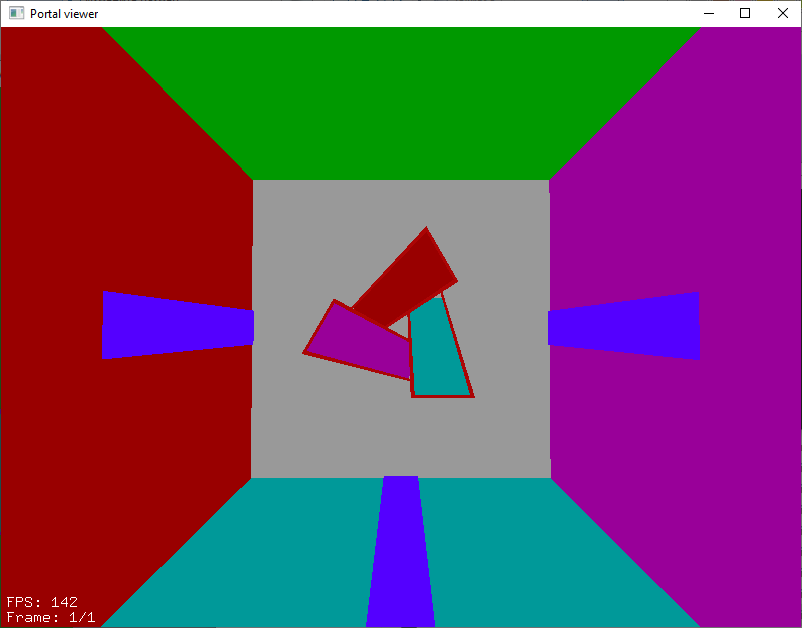
\includegraphics[width=.48\textwidth]{img/19.png}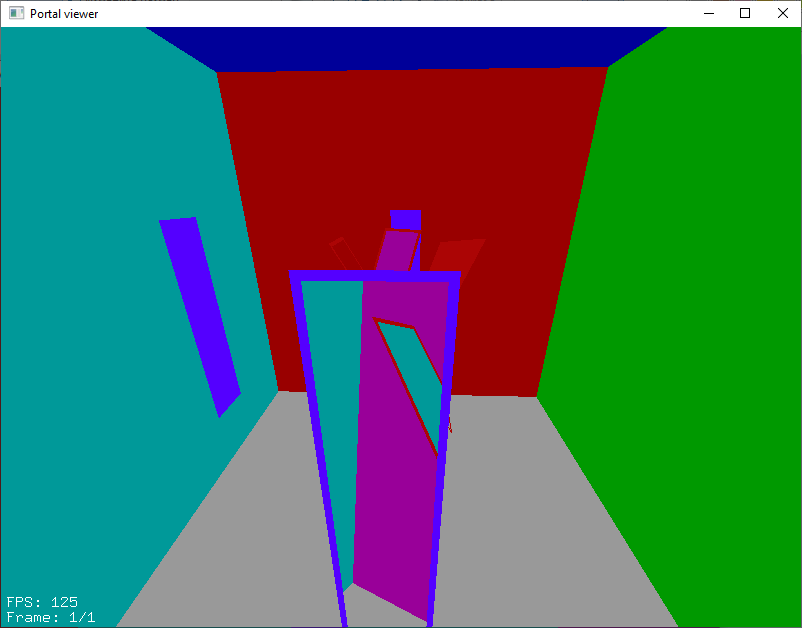
\includegraphics[width=.48\textwidth]{img/20.png}
\end{center}

\subsection{Работа освещения}

\begin{center}
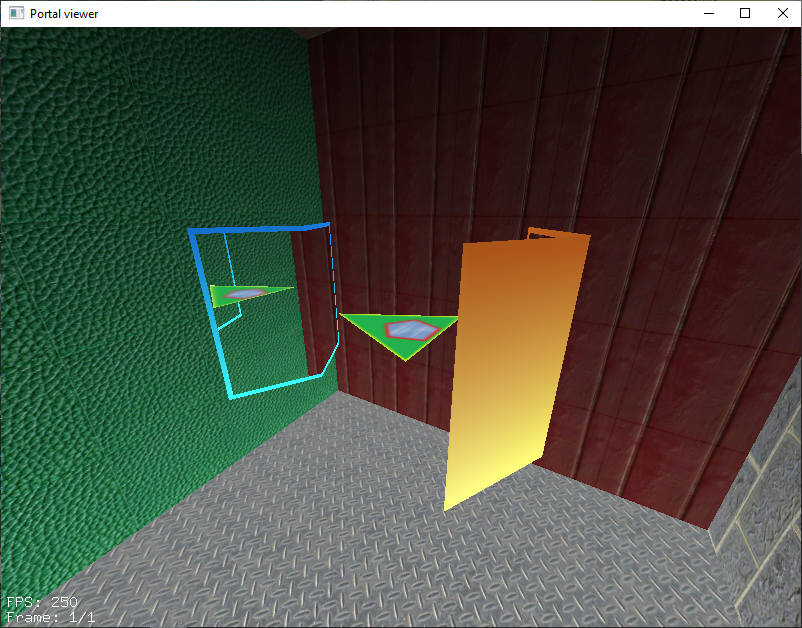
\includegraphics[width=.48\textwidth]{img/21.png}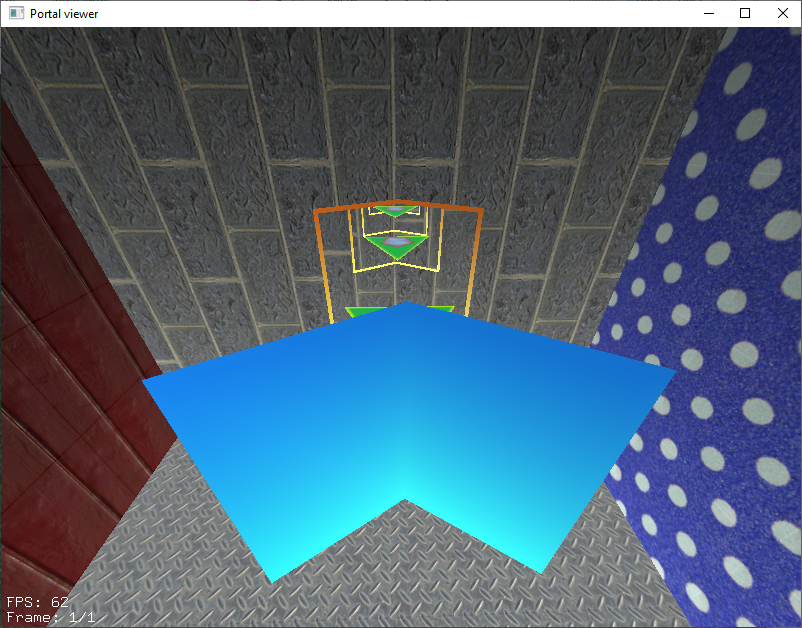
\includegraphics[width=.48\textwidth]{img/22.png}
\end{center}

\section{Код программы}

\subsection{Файлы заголовков}

\mycodeinput{c++}{code/fragment.h}{fragment.h}
\mycodeinput{c++}{code/framebuffer.h}{framebuffer.h}
\mycodeinput{c++}{code/opengl_common.h}{opengl\_common.h}
\mycodeinput{c++}{code/plane.h}{plane.h}
\mycodeinput{c++}{code/scene_reader.h}{scene\_reader.h}
\mycodeinput{c++}{code/shader.h}{shader.h}

\subsection{Исходные файлы}

\mycodeinput{c++}{code/main.cpp}{main.cpp}
\mycodeinput{c++}{code/fragment.cpp}{fragment.cpp}
\mycodeinput{c++}{code/framebuffer.cpp}{framebuffer.cpp}
\mycodeinput{c++}{code/opengl_common.cpp}{opengl\_common.cpp}
\mycodeinput{c++}{code/plane.cpp}{plane.cpp}
\mycodeinput{c++}{code/scene_reader.cpp}{scene\_reader.cpp}
\mycodeinput{c++}{code/shader.cpp}{shader.cpp}

\subsection{Шейдеры}

\mycodeinput{c++}{code/draw.fragment.glsl}{draw.fragment.glsl}
\mycodeinput{c++}{code/draw.vertex.glsl}{draw.vertex.glsl}
\mycodeinput{c++}{code/drawpoly.fragment.glsl}{drawpoly.fragment.glsl}
\mycodeinput{c++}{code/drawpoly.vertex.glsl}{drawpoly.vertex.glsl}
\mycodeinput{c++}{code/merge.fragment.glsl}{merge.fragment.glsl}
\mycodeinput{c++}{code/merge.vertex.glsl}{merge.vertex.glsl}

\subsection{Сцены}

В целях экономия места написана только одна сцена:

\mycodeinput{js}{code/volumetric_portal_with_textures.json}{volumetric\_portal\_with\_textures.json}